%!TEX root = ../thesis.tex
% створюємо розділ
\chapter{Генерація випадкових чисел у смарт картах}
\label{chap:theory}

Смарт-картки широко використовуються в різних галузях, таких як банківська справа, телекомунікації, посвідчення особи та інші, де потрібна генерація унікальних і безпечних даних для шифрування, підписів та інших криптографічних сервісів. У зв'язку з цим, дослідження генерації псевдовипадкових чисел (ПВЧ) у смарт-картках не таке вже й безпідставне. 


Розглянемо, як TRNG реалізовано в комп'ютерах загального призначення, і як їхня архітектура може бути адаптована для використання в смарт-картках. Модифікації моделі генератора TRNG, реалізованих на Java Card, аналізуються з погляду продуктивності та випадковості за використання набору статистичних тестів NIST SP 800-22.


Важливою мотивацією є необхідність забезпечення безпеки генерованих послідовностей, особливо в умовах обмежених ресурсів смарт-карток. Потрібно звертати увагу на критерії безпеки, що висуваються до генераторів PRNG, включно з вимогами Common Criteria та AIS31. Поглянемо на різні аспекти генерації PRNG у смарт-картках, модифікації наявних моделей та їхній аналіз для забезпечення безпеки та ефективності в контексті криптографічних застосувань.


\section{Пристрій смарт-картки}

Смарт-картка являє собою пристрій з обмеженими ресурсами, включно з центральним процесором, пам'яттю тільки для читання (ПЗП), оперативною пам'яттю (ОЗП), програмованою пам'яттю для читання, яка електрично стирається (EEPROM), і криптопроцесором. Дані зберігаються в ПЗП і EEPROM, де останнє являє собою обмежений за циклами ресурс, що підкреслює необхідність ефективного захисту від атак.


Обмеження смарт-карт на генератори псевдовипадкових чисел пов'язані з обмеженими джерелами ентропії. На відміну від комп'ютерів, де джерела ентропії більш різноманітні, у смарт-картах ці джерела обмежені. Апаратні обмеження також включають обмежений обсяг пам'яті та обмежені обчислювальні можливості. У зв'язку з цим, кращим рішенням є використання апаратних генераторів псевдовипадкових чисел. Існуючі генератори випадкових чисел у смарт-картках зазвичай засновані на регістрах зсуву з лінійним зворотним зв'язком (LFSR) \cite{kar2019general}, але такі послідовності не забезпечують достатнього рівня безпеки для криптографічного використання. Крім того, обмеження стандарту FIPS 140-2 впливають на вибір програмних реалізацій TRNG у смарт-картках. Важливим моментом є відсутність можливості противника надавати або маніпулювати вхідними даними TRNG, що забезпечує стійкість до передбачень і запобігає розкриттю інформації про внутрішній стан генератора. Такі обмеження смарт-карток вимагають ретельного підходу до розробки та забезпечення безпеки генераторів псевдовипадкових чисел.

\section{Загальна модель для TRNG}

Розглянемо загальну модель для генераторів псевдовипадкових чисел (TRNG).

\begin{enumerate}
    \item \textbf{Узагальнена модель TRNG:}
    \begin{enumerate}
        \item Розроблено загальну модель, враховуючи бажані властивості та рекомендації з різних джерел.
        \item Модель включає в себе функцію форматування введення (IFF), алгоритм-генератор (GA), генератор оновлення насіння (SUG), і функцію форматування виходу (OFF).
    \end{enumerate}

    \item \textbf{Кроки обробки:}
    \begin{enumerate}
        \item IFF: Витягує початкове значення з циклічного буфера (CB), що слугує джерелом ентропії. Обробляє дані, задовольняючи вимогам алгоритму-генератора.
        \item GA: Приймає вихідні дані IFF і обробляє їх з використанням криптографічної функції (Hash, MAC, DES, AES та ін.).
        \item SUG: Генерує значення для оновлення насіння і повертає його IFF, використовуючи XOR з виходом GA.
        \item SFUF: Виконує оновлення насіння, отримуючи значення оновлення і виконуючи XOR з виходом SUG.
        \item OFF: Приймає вихідні дані GA і форматує їх відповідно до вимог користувача або програми.
    \end{enumerate}

    \item \textbf{Ітераційний процес:}
    \begin{enumerate}
        \item Другий раунд включає кроки 1 і 2, але вихід GA не передається SUG.
        \item Додаткова ітерація (OFF) виконується для приховування значення, яке використовується для оновлення затравочного файлу.
    \end{enumerate}

    \item \textbf{Формування Псевдовипадкових Чисел:}
    \begin{enumerate}
        \item Функція форматування виходу (OFF) перетворює вихідні дані GA в бажаний вихідний сигнал.
    \end{enumerate}
\end{enumerate}

\section{Результати експериментів}


Тепер надамо результати роботи шести реалізацій генераторів псевдовипадкових чисел (TRNG) для смарт-карток на основі представленої загальної моделі від авторів статті. Реалізації різняться не тільки використовуваним алгоритмом генератора (GA), а й пов'язаними з ним функціями. Весь експеримент проводився на Java Card, як на симуляторі, так і на реальних картах.


\textbf{Експериментальне середовище:}
\begin{itemize}
    \item Тести проведено на симуляторі (Java Card simulator JCWDE) і реальних смарт-картках.
    \item Експерименти підтримують використання різних криптографічних алгоритмів як GA.
\end{itemize}


\textbf{Вимірювання продуктивності:}
\begin{itemize}
    \item Продуктивність тестованих TRNG оцінювалася на Java Card Virtual Machine.
    \item Експериментальна матриця продуктивності включає результати вимірювань для кожної реалізації на двох 16-бітних Java-картах.
\end{itemize}


\textbf{Оцінка розмірів:}
\begin{itemize}
    \item Розміри реалізацій в EEPROM представлені в таблиці. У комерційній реалізації в EEPROM зберігається тільки файл приманки, а код ГПСЧ, частина операційної системи смарт-картки, міститься в ПЗП.
\end{itemize}


\textbf{Тести Продуктивності:}
\begin{itemize}
    \item Смарт-картки вставлялися в зчитувач, підключений до осцилографа.
    \item Тестовий додаток вибирав TRNG і запитував 128 біт випадкового числа.
    \item Вимірювався час від запиту до отримання вихідного сигналу, а потім бралося середнє значення для оцінки продуктивності.
\end{itemize}


\textbf{Результати:}
\begin{itemize}
    \item Генератори на основі хеша показали найкращу продуктивність серед реалізованих TRNG.
    \item Матриця продуктивності та статистичні тести для випадковості надають повний огляд характеристик кожної реалізації.
\end{itemize}

\begin{figure}[h]
  \centering
  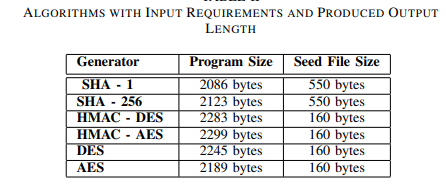
\includegraphics[width=0.8\textwidth]{IMAGES/03.png}
  %\caption{Подпись к картинке}
  \label{fig:fig1}
\end{figure}

\begin{figure}[h]
  \centering
  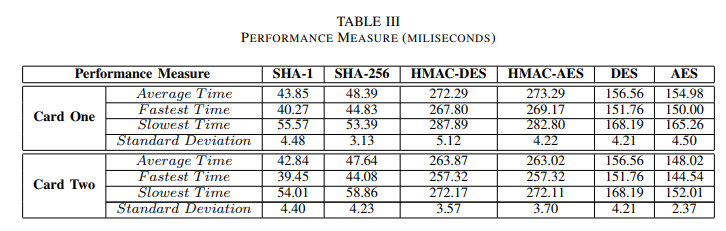
\includegraphics[width=0.8\textwidth]{IMAGES/04.png}
  %\caption{Подпись к картинке}
  \label{fig:fig1}
\end{figure}

\begin{figure}[h]
  \centering
  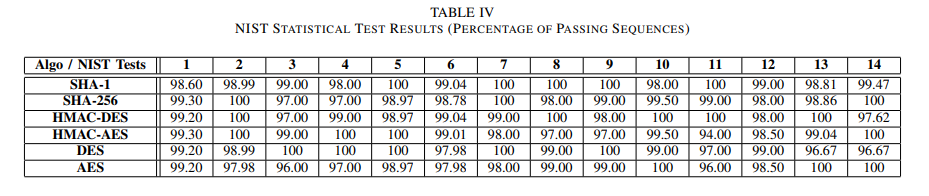
\includegraphics[width=0.8\textwidth]{IMAGES/05.png}
  %\caption{Подпись к картинке}
  \label{fig:fig1}
\end{figure}

\begin{figure}[h]
  \centering
  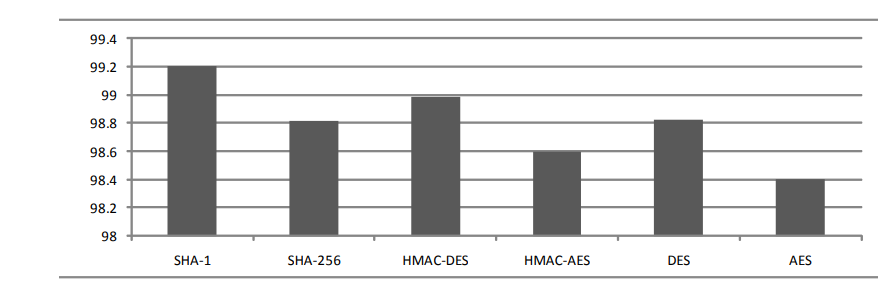
\includegraphics[width=0.8\textwidth]{IMAGES/06.png}
  \caption{Graph Depicting Average Percentage of Passing Sequence Across NIST Statistical Test Results (Table IV)}
  \label{fig:fig1}
\end{figure}